\documentclass{article}

\usepackage{notes}

\title{Estimating the mana of magical matrix product operators}
\author{Siddhartha Harmalkar}
\date{November 2020}

\begin{document}
\maketitle

\tableofcontents

\section{Introduction}

Quantum error correction codes based on stabilizer circuits provide a robust theory of fault-tolerant, albeit non-universal, quantum computation. To achieve universal quantum computation, an extra resource of non-stabilizer gates or states prepared using such gates - ``magic'' states - can be injected into the system. A resource theory of this model of universal quantum computation has been developed to quantify the amount of magical resource required to perform tasks such as preparing a magical state on a quantum computer \cite{Veitch_2014}. 

Using this resource theory to quantify such tasks involves the computation of measures of magic - the \textit{mana} and \textit{relative entropy of magic}, for example \cite{Veitch_2014} - which are exponentially hard to compute in the size of the system. Here we introduce a new measure which allows for a polynomial-time computation when applied to matrix product operators.

%Stabilizer codes have been used to construct proposals of solvable toy models of holographic duality, by noting that the structure of a class of codes in which the logical and physical qubits are related by a tensor network resembles that of holographic bulk reconstruction \cite{Pastawski_2015}. However, these models are conjectured to miss features of a true holographic state \cite{Cui_2019} in an AdS/CFT duality, which we might be able to quantify using this resource theory. 

\section{Approximating the mana $\mathcal M$ with a related quantity $\mathcal N$}

Stabilizer states are the only pure states with non-negative Wigner function in Hilbert spaces of odd dimension \cite{Gross_2006}. All mixtures of stabilizer states therefore have non-negative Wigner function\footnote{However, there do exist mixed states with non-negative Wigner function which are not mixtures of stabilizer states - see section V of \cite{Gross_2006}}. Moreover, the degree to which a state's wigner function is negative gives us information about how much magical resource is required to create it: The \textit{mana} of a mixed state
\begin{equation}\mathcal M(\rho)=\ln\sum_{u}\left |W_\rho(u)\right|\end{equation}
quantifies the amount of magical resource needed to prepare magical states using procedures such as magical state distillation \cite{Veitch_2014}, where $W_u(\rho)$ is the Wigner function of the state $\rho$ - see Section \ref{sec:wigner_fct} for details. Computation of the mana of an arbitrary state is exponentially hard in the size of the system, as it requires us to know $W_u(\rho)$ for all $d^{2n}$ possible strings $u\in\mathbb Z_d^{2n}$, an intractable computation for large system sizes. 

Instead of calculating the mana, we can approximate the magic of a state with the quantity
\begin{equation}\mathcal N(\rho)=\sqrt{\sum_{u\in N(\rho)}W_{\rho}(u)^2},\end{equation} where $N(\rho)$ is the set of strings satisfying $W_u(\rho)<0$. While $\mathcal N$ does not satisfy the same properties as $\mathcal M$ which would allow us to use it to quantify the amount of resource needed for tasks such as magic state distillation, it is clearly larger for more states with larger mana, and is emperically highly correlated with $\mathcal M$ for a generic mixed state:

\begin{figure}[H]
\centering
\subfloat[$\mathcal M$ vs. $\mathcal N$ for mixed single qutrit states]{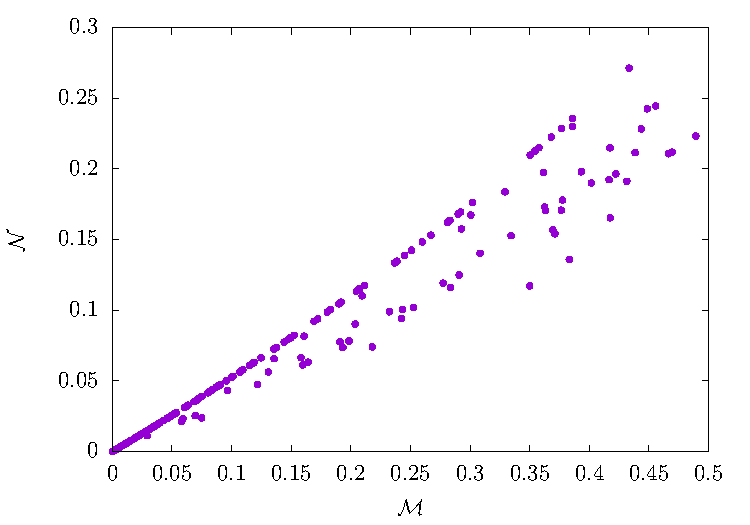
\includegraphics[width=0.45\linewidth]{magik_1}}\hspace{1.5em} \subfloat[$\mathcal M$ vs. $\mathcal N$ for mixed two qutrit states of two types - product states and arbitrary mixed states]{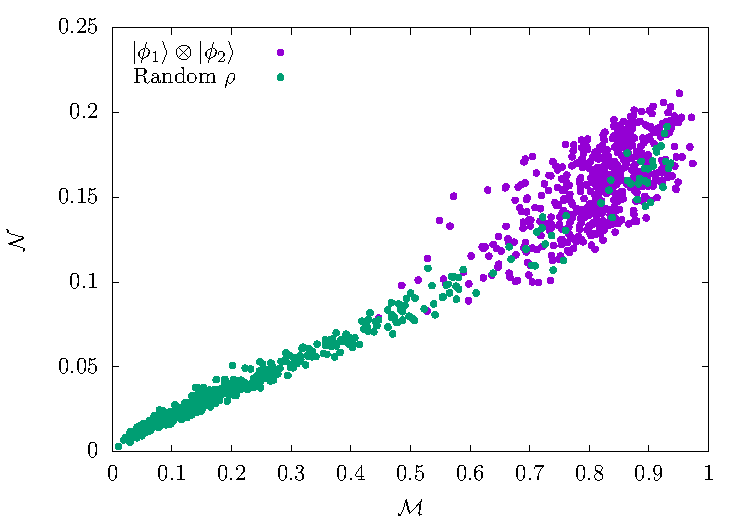
\includegraphics[width=0.45\linewidth]{magik_2}}
\caption{Comparison of $\mathcal M$ and $\mathcal N$ on a variety of mixed states. Each mixed state in the plots is randomly generated according to the algorithm described in Section \ref{sec:random_state_gen} out of $N$ randomly sampled pure states, where $N$ was uniformly sampled between 1 and 20.}
\end{figure}

We find that $\mathcal N$ is much easier to work with than $\mathcal M$\footnote{This is reminiscent of how the standard deviation of a distribution, $\mathrm{E}[(X-\mathrm{E}[X])^2]^{1/2}$, is an easier quantity to work with than the more direct measure of the degree to which samples deviate from the mean: $\mathrm{E}[|X-\mathrm{E}[X]|]$}. In particular, we can efficiently approximate $\mathcal N$ by noticing that it is the distance between the state $\rho$ and the space of operators\footnote{Note that not all operators satisfying $W_u(\rho)\geq 0\ \forall u$ represent states - only those with $\Tr\rho=1$. Hermiticity is gauranteed, though, due to the fact that $W_u(\rho)\in \mathbb R$.} with non-negative Wigner function:
\begin{equation}\mathcal N(\rho)=\underset{\mathcal M(\sigma)=0}{\min}d(\rho,\sigma),\end{equation}
where
\begin{equation}d(\rho,\sigma)\equiv \sqrt{\sum_{u\in \mathbb Z_d^{2n}} \left(W_{\rho}(u)-W_{\sigma}(u)\right)^2}\end{equation}
is the distance between two operators when viewed as vectors in the space of Wigner function coefficients. Therefore, we can approximate $M_2(\rho)$ by minimizing $d(\rho,\sigma)$ in the space of non-negative Wigner function operators $\sigma$. 

\section{Efficient approximation of $\mathcal N$ for a matrix product operator}

Given a local operator basis $A_i$ of the space dual to the Hilbert space $\mathcal H$, the tensor product $A_{i_1}\otimes A_{i_2}\otimes\cdots\otimes A_{i_n}$ forms a basis of the $n$-site dual space $(\mathcal H^*)^{\otimes n}$. A matrix product operator (MPO) is an operator $\mathcal O\in (\mathcal H^*)^{\otimes n}$ of the form
\begin{equation}\mathcal O=\sum_u\left(\sum_{\alpha}M_{\alpha_1\alpha_2}^{(1)u_1}M_{\alpha_2\alpha_3}^{(2)u_2}\cdots M_{\alpha_n\alpha_{n+1}}^{(n)u_n}\right)A_{u_1}\otimes A_{u_2}\otimes\cdots\otimes A_{u_n},\end{equation}
where $\{M^{(i)u}\}_{u=1}^d$ is a collection of $d$ matrices ``at site $i$'', indexed by $u$, with dimension\footnote{The first and last matrices have dimension $1\times D$ and $D\times 1$, respectively - $\alpha_1$ and $\alpha_{n+1}$ are dummy indices which only take on one value} $D\times D$. $D$ is referred to as the \textit{bond dimension} of the MPO.

% The mana can be written as $\mathcal M(\rho)=\sum_{u\in P(\rho)}W_u(\rho)-\sum_{u\in N(\rho)}W_u(\rho)$, where $P(\rho)$ and $N(\rho)$ are the set of strings satisfying $W_u(\rho)\geq 0$ and $W_u(\rho)<0$, respectively. If we knew $P(\rho)$ and $N(\rho)$, we could exploit the matrix product structure of an MPO $\rho$ to compute the mana in polynomial time in the onsite hilbert space dimension $d$ and the bond dimension $\chi$. The procedure would be to write the MPO in the phase space operator basis (see Section \ref{sec:phase_space}), in which the sum of values of the Wigner function is simply the sum of values of the coefficients of $\rho$ in the local operator basis. This can be written as a contraction of $\rho$ with an MPO with matrices $M^{(i)u_i}=1$, a calculation that can be done in $dD^3$ time.
% 
% However, we we don't know the structure of $N(\rho)$ for an arbitrary MPO. So we need to use a different quantity to get a handle on the magic of MPOs for large system sizes.

The structure of matrix product operators can be exploited to reduce computational costs which are generically exponential in the $d$ to ones which are linear in the $d$ and polynomial in $D$. The procedure of estimating $\mathcal N(\rho)$ outlined above allows for such a reduction in computation time if $\rho$ is an MPO and the variational state $\sigma$ is also an MPO, as we can efficiently perform the contractions required in the computation of $d(\rho,\sigma)$ and its derivatives with respect to the degrees of freedom in $\sigma$ at a single site - see Section \ref{sec:contractions}

The procedure is then to sweep through sites in a DMRG-like fashion, optimizing $d(\rho,\sigma)$ with respect to the degrees of freedom at each site in $\sigma$, under the constraint that $\sigma$ remains in the space of states with non-negative Wigner function:

\paragraph{Algorithm for approximating $\mathcal N(\rho)$:} Given a matrix product operator $\rho=\sum_\alpha \otimes_k M^{(k)u_k}_{\alpha_k\alpha_{k+1}} A_k$ with bond dimension $D_\rho$, where $A_i$ are the phase space operators\footnote{If $\rho$ is represented in a different basis, perform a local change of basis to find its Wigner representation first: Let $\rho=\sum_\alpha \otimes_k M^{(k)u_k}_{\alpha_k\alpha_{k+1}} B_k$, where $B_k$ is some local operator basis. Then this consists of performing the change of basis $\rho^{(i)u}_{\alpha\beta}=\sum_v U_{uv}\rho^{(i)v}_{\alpha\beta}$, where $U_{uv}=\Tr[A_uB_v]$} \eqref{eq:phase_space_ops}:

\begin{enumerate}
\item Let $\sigma=\sum_{u,\alpha_i} \otimes_k\ \sigma^{(k)u_k}_{\alpha_k\alpha_{k+1}} A_{u_k}$ be a random MPO with bond dimension $D_\sigma$ such that $\sigma^{(k)u}_{\alpha\beta}\ \forall k\in \mathbb Z_n, u\in \mathbb Z_d^{2n},\alpha,\beta\in Z_{D_\sigma}$.
\item Set $i\leftarrow 1$. While $i\leq n$:
	\begin{enumerate}
		\item Precompute the contractions required in the computation of the derivatives $\frac{\partial d(\rho,\sigma)}{\sigma^{(i)a}_{\alpha\beta}}$ - see Section \ref{sec:contractions}.
		\item Let $\mathcal F$ be the set of $d\times D_\sigma\times D_\sigma$ sized tensors\footnote{Since the first and last bond indices are dummy indices, the tensors have size $d\times 1\times D_\sigma$ for $i=1$, and $d\times D_\sigma\times 1$ for $i=n$} with non-negative elements: $x\in\mathcal F\Rightarrow x^u_{\alpha,\beta}\geq 0\ \forall u\in\mathbb Z_d, \alpha,\beta\in\mathbb Z_{D_\sigma}$, and $\hat \sigma(x)$ be the function which replaces the matrix in $\sigma$ at site $i$ with the matrix $x$:
		\begin{equation}\hat \sigma:x\in \mathcal F\mapsto\sum_u\left(\sum_{\alpha}\sigma_{\alpha_1\alpha_2}^{(1)u_1}\cdots \sigma_{\alpha_{i-1}\alpha_i}^{(i-1)u_{i-1}}x^{u_i}_{\alpha_i\alpha_{i+1}}\sigma_{\alpha_{i+1}\alpha_{i+2}}^{(i+1)u_{i+1}}\cdots\sigma_{\alpha_L\alpha_{L+1}}^{(n)u_n}\right)A_{u_1}\otimes A_{u_2}\otimes\cdots\otimes A_{u_n}\end{equation}
		\item Solve the constrained optimization problem $\sigma^{(i)*}=\underset{x\in\mathcal F}{\operatorname{argmin}}\ d(\rho,\hat \sigma(x))$ numerically, using a procedure such as \cite{bfgs_large_scale}.
		\item  $\sigma^{(i)}\leftarrow \sigma^{(i)*}$
		\item $i\leftarrow i+1$
		\end{enumerate}
	\item Repeat step 2 until $d(\rho,\sigma)$ asymptotes\footnote{Note that optimization algorithms might appear to asymptote but can later perform better if allowed to continue}
	\item Increase the bond dimension $D_\sigma$. Repeat steps 2 and 3 until $d(\rho,\sigma)$ asymptotes with respect to bond dimension (or the computational resources required in step 2 become intractable).
\end{enumerate}


\section{Caveats}

A few things should be noted about this optimization:

\begin{itemize}
	\item Even if the optimization is done perfectly, the final distance $d(\rho,\sigma)$ will only be an upper bound for $\mathcal N(\rho)$. This is because the set of states we can reach in our optimization algorithm is only a subset of the set of operators with non-negative Wigner function, due to the fact that $\sigma$ has a matrix product structure with fixed bond dimension and $\sigma^{(i)u_i}_{\alpha\beta}\geq 0\ \forall i,u_i,\alpha,\beta$, which is more restrictive than the requirement that $\sigma$ have non-negative Wigner function representation, i.e $W_u(\sigma)=\sum_\alpha \prod_i \sigma^{(i)u_i}_{\alpha_i,\alpha_{i+1}}\geq 0\ \forall u\in \mathbb Z_d^{2n}$. In practice, we alleviate the first restriction slightly by using larger bond dimensions until we either see our estimate for $\mathcal N$ asymptote or we run out of resources.
	\item The space of MPOs with fixed bond dimension is not convex - adding two MPOs generally increases the bond dimension of the MPO. This means that our contrained optimization problem might settle on local minima. 
\end{itemize}

\pagebreak

\section{Results}

Running the above algorithm with the L-BFGS-B constrained optimization method (As seen below, the L-BFGS-B method \cite{bfgs,bfgs_large_scale} for constrained optimization works well in practice, outperforming an interior point method solver (``trust-constr'') and a sequential least squares quadratic programming method (``SLSQP'')) on a random magical mixed state $\rho$ generated using $N=20$ randomly sampled pure states as described in Section \ref{sec:random_state_gen} shows that the approximation for $\mathcal N(\rho)$ can get better with larger bond dimension, but starts to require more sweeps to asymptote after a certain point.

\begin{figure}[H]
\centering
\subfloat[Distance between a randomly generated 2-site MPO and the optimized MPO vs. sweeps for various optimizers.]{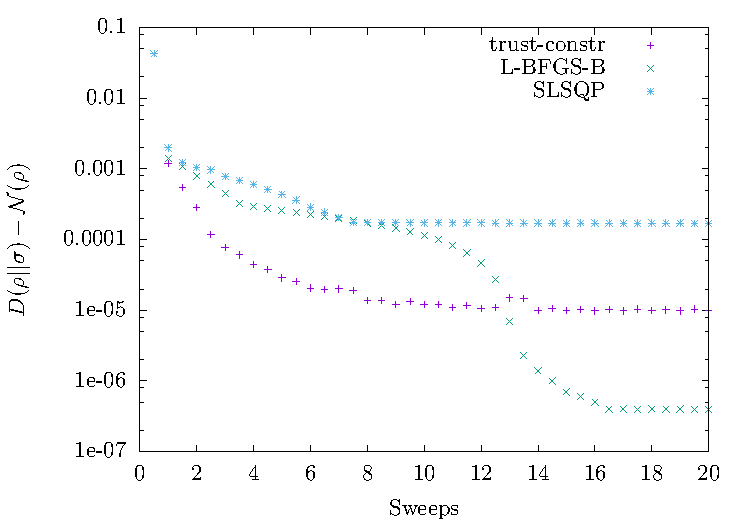
\includegraphics[width=0.45\linewidth]{optimizer_comparison}}
\subfloat[Runs with L-BFGS-B for varying bond dimensions]{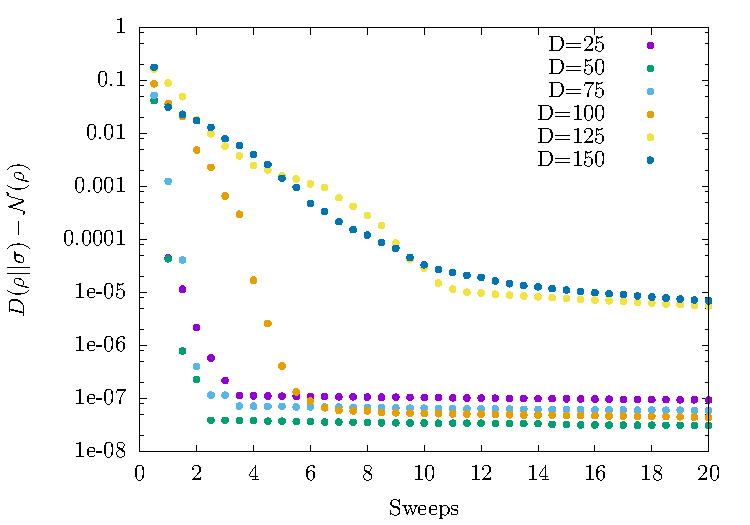
\includegraphics[width=0.45\linewidth]{bond_dim}}
\caption{Results from running the algorithm for approximating $\mathcal N(\rho)$ of a random mixed state $\rho$. Each run consists of 20 sweeps, and generates 40 points due to two optimizations being done during each sweep - one for each site.}
\end{figure}

\section{Next steps}

We need to analyze optimization function on a variety of test cases to understand how it performs. for small $n$, we can exactly compute the true value of the optimal cost function and compare. Some ideas of families of states to look at:
\begin{itemize}
\item $S_\rho(\alpha)=\alpha\rho+\frac{(1-\alpha)}{d}I$, where $\rho$ is a random pure state. As we vary $\alpha$ from 0 to 1, the state should start to gain more magic as soon as it clears the stabilizer hull. Sampling a set of random $\rho$ uniformly and computing the average and standard deviation of the error in the result after optimization as a function of $n$ will give a good estimate of how well the optimizer does as the system size increases. 
\item $S_{a,b}(\alpha)=aS_1+bS_2-\alpha I/d^n$: Here the idea is to mix two stabilizer states  $S_1$ and $S_2$ and walk in the negative direction of identity.  This is a good test because the distance $d(S_{a,b}(\alpha),I/d^n)$ should be linear in $\alpha$ even for large $n$.
\item MPSs with truncated bond dimensions: Create a random state, turn it into an MPS with truncated bond dimension, or just do SVDs at each site and project onto the first few singular components. Truncate enough so that the mana is tractable even at large $n$, to compute the error in optimization exactly.
\end{itemize}

\section{Future work}

\begin{itemize}
\item Extend results to larger system sizes
\item Estimate the magic of the ground state of a CFT, such as the spin-1 Potts model near criticality, for large system sizes
\item Improve the algorithm for approximating $\mathcal N(\rho)$. Some ideas for doing so:
	\begin{itemize}
	\item Understand why the constrained optimization procedure requires significantly more sweeps to converge when the bond dimension of $\sigma$ is increased
	\item Understand why the value which the procedure asymptotes to does not always decrease with increasing bond dimension (what's most likely happening is that the optimization is taking so long to asymptote that it seems to asymptote early at a non-optimal value)
	\item Initialize the optimization with a clever initial condition, which might help alleviate the issues above
	\item Relax the constraint that all matrix elements of $\sigma^{(i)u}$ be non-negative, while ensuring that $W_u(\sigma)>0\ \forall u\in \mathbb Z_d^{2n}$. This would allow for better approximation of $\mathcal N(\rho)$
	\end{itemize}
\item Attempt to optimize the \textit{relative entropy} \cite{Veitch_2014} $\rho \log \rho - \rho \log \sigma$ with the constraint that $\sigma$ is a stabilizer state, which can more directly quantify the magic of $\rho$. This would require including a normalization constraint in the optimization. It's not clear how to ensure that $\sigma$ is a stabilizer state during the optimization, however, due to the fact that some states with nonnegative Wigner representation are not stabilizers, so we would most likely have to just approximate the stabilizer hull with the space of nonnegative Wigner representation states as well. 
\end{itemize}



\pagebreak

\appendix

\section{Stabilizer formalism}

\subsection{Heisenberg-Weyl operator basis}

Mixed states of qubits can be nicely represented using the familiar pauli matrices $\sigma_i$ of 2-component quantum mechanics, which can be used to construct a set of $4$ operators which form a basis of hermitian $2\times 2$ matrices: $\sigma_\alpha=\frac{1}{2}(1,\sigma_i).$ The factor of $\frac{1}{2}$ gives orthonormality with respect to the frobenius norm: $(\sigma^i)^2=1$ and $\Tr \sigma^i=0$ imply that $\Tr[(\sigma_\alpha)^\dagger\sigma_\beta]=\delta_{\alpha\beta}$, allowing for any mixed state to be written as $\rho=\sum_\alpha\Tr[\sigma_\alpha\rho]\sigma_\alpha$. A basis for mixed states of $n$ qubits is then given by ``strings'' of pauli matrices tensored together: the string $u=(u_1,u_2,\ldots,u_n)\in \mathbb Z_4^{n}$ indexes the basis element $\otimes_{i=1}^n \sigma_{u_i}$.

For a general qudit, a set of $d^2$ operators is needed to decompose qudit states. If $d>2$ is prime, one choice of operators is the so-called \textit{generalized pauli matrices} or \textit{Heisenberg-Weyl operators}:
\begin{equation}T_{u}=\omega^{-(d+1)ab/2}Z^{a}X^{b}=\omega^{-2^{-1}ab}Z^aX^b,\end{equation}
where $u=(a,b)\in \mathbb Z_d\times \mathbb Z_d$, $\omega=e^{2\pi i/d}$ is the $d$-th root of unity, $2^{-1}=\frac{d+1}{2}$ is the multiplicative inverse of $2$ modulo $d$ if $d$ is odd (which it is for prime $d>2$), and $X$ and $Z$ are the \textit{boost} and \textit{shift} operators, respectively, whose action on the computational basis is
\begin{equation}X\left|k\right>=\left|k\oplus 1\right>\text{ and }Z\left|k\right>=\omega^k\left|k\right>,\end{equation}
where $\oplus$ denotes addition modulo $d$. Note that any operation on $a$ and $b$ can be thought of as being modulo $d$, because $\omega^d=X^d=Z^d=1$:
\begin{equation}X^d\left|k\right>=\left|k\oplus d\right>=\left|k\right>, Z^d\left|k\right>=\omega^d\left|k\right>=\left|k\right>\end{equation}
The boost and shift operators are unitary:
\begin{equation}\left <i\right|X^\dagger X\left |j\right>=\left <i\oplus 1|j\oplus 1\right>=\delta_{ij}\Rightarrow X^\dagger=X^{-1},\ \left <i\right|Z^\dagger Z\left |j\right>=\left <i\right |\omega^{-i}\omega^j\left|j\right>=\omega^{j-i}\delta_{ij}=\delta_{ij}\Rightarrow Z^\dagger=Z^{-1}\end{equation}
and have commutation structure $[Z,X]=(\omega-1)XZ$:
\begin{equation}\label{eq:XZ} XZ\left|k\right>=\omega^k\left |k\oplus 1\right>,\ ZX\left|k\right>=\omega^{k+1}\left |k\oplus 1\right>\Rightarrow ZX=\omega XZ\end{equation}
They are orthonormal up to a factor of $d$: 
\begin{equation}\label{eq:boost_shift_trace} \Tr[X^a]=\sum_k \left<k|k\oplus a\right>=d\delta_{a,0},\ \Tr[Z^b]=\sum_k (\omega^b)^k=d\delta_{b,0}+\frac{1-\omega^{bd}}{1-\omega^b}(1-\delta_{b,0})=d\delta_{b,0}\Rightarrow \Tr[Z^aX^b]=d\delta_{a,0}\delta_{b,0},\end{equation}
which implies that the generalized pauli operators satisfy $\Tr[T_{(a,b)}]=d\delta_{a,0}\delta_{b,0}$ and
\begin{align}\label{eq:generalized_pauli_prod_tr}\Tr[T_{(a,b)}T_{(a',b')}]&=\omega^{-2^{-1}ab}\omega^{-2^{-1}a'b'}\Tr[Z^aX^bZ^{a'}X^{b'}]=\omega^{-2^{-1}(ab+a'b')+a'b}\Tr[Z^{a+a'}X^{b+b'}]\\&=\omega^{-2^{-1}(b(a+a')+a'(b+b'))}d\delta_{a,-a'}\delta_{b,-b'}=d\delta_{a,-a'}\delta_{b,-b'}\end{align}

For a system of $n$ qudits, the generalized pauli matrices are built up from their single qudit analogs in the same way as the pauli matrices are, and can be indexed by a string $u=(a_1,b_1,a_2,b_2,\ldots,a_n,b_n)\in \mathbb Z_d^{2n}$: 

\begin{equation}T_u=\otimes_{i=1}^n T_{(a_i,b_i)}.\end{equation}

The generalized pauli matrices, unlike the pauli matrices, are unitary - they are composed of a product of unitary operators. They are not hermitian and therefore do not form an orthonormal basis of operators that can be used to represent density matrices. However, they fail to be hermitian in a very specific way: The hermitian conjugate of a generalized pauli matrix is another generalized pauli matrix:

\begin{equation}T_{(a,b)}^\dagger=\left(\omega^{-2^{-1}ab}Z^aX^b\right)^\dagger=\left(\omega^{-2^{-1}ab+ab}X^bZ^a\right)^\dagger=\omega^{-2^{-1}ab}Z^{-a}X^{-b}=T_{(-a,-b)},\end{equation}
where we've used the fact that $X$ and $Z$ are unitary and are related to each other by \eqref{eq:XZ}, which implies that $Z^aX^b=\omega^{ab}X^bZ^a$. 

This means that the sum of all generalized pauli matrices is hermitian:
\begin{equation}\left(\sum_{(a,b)}T_{(a,b)}\right)^\dagger=\sum_{(a,b)}T_{(a,b)}^\dagger=\sum_{(a,b)}T_{(-a,-b)}=\sum_{(a',b')}T_{(a',b')}\end{equation}
This fact will allow us to construct a basis of hermitian operators.

\subsection{Phase space operator basis}

\label{sec:phase_space}

The \textit{phase space operators} for are
\begin{equation}\label{eq:phase_space_ops}A_u=\frac{1}{d^n}T_u\left(\sum_{v\in\mathbb Z_d^{2n}} T_v\right)T_u^\dagger,\end{equation}
and satisfy the property
\begin{equation}A_u=\otimes_{i=1}^n A_{(a_i,b_i)}.\end{equation}
They are hermitian, as they are formed by unitary conjugation of the hermitian operator $\sum_u T_u$. The single qudit operators have unit trace:
\begin{equation}\label{eq:phase_space_trace}\Tr[A_u]=\frac{1}{d}\Tr[T_u^\dagger (\sum_v T_v) T_u]=\frac{1}{d}\Tr[\sum_v T_v]=\frac{1}{d}\Tr[1]=1,\end{equation}
and are trace orthonormal up to a factor of $d$:
\begin{align}\Tr[A_{(a,b)}A_{(a',b')}]&=\frac{1}{d^2}\sum_{i,j,i',j'}\Tr[T_{(a,b)}T_{(i,j)}T_{(a,b)}^\dagger T_{(a',b')}T_{(i',j')}T_{(a',b')}^\dagger]=\frac{1}{d^2}\sum_{i,j,i',j'}\omega^{ib-aj+i'b'-a'j'}\Tr[T_{(i,j)}T_{(i',j')}]\\&=\frac{1}{d}\sum_{i,j}\omega^{ib-aj-ib'+a'j}=\frac{1}{d}\sum_i \omega^{i(b-b')}\sum_j \omega^{j(a'-a)}=d\delta_{a,a'}\delta_{b,b'},\label{eq:phase_space_norm}\end{align}
where we've used the fact that
\begin{equation}T_{(a,b)}T_{(a'b')}=\omega^{-2^{-1}(ab+a'b')}Z^aX^bZ^{a'}X^{b'}=\omega^{-2^{-1}(ab+a'b')}\omega^{a'b-ab'}Z^{a'}X^{b'}Z^aX^b=\omega^{a'b-ab'}T_{(a',b')}T_{(a,b)}.\end{equation}

\subsection{Wigner function representation of a mixed state}

\label{sec:wigner_fct}

The \textit{wigner function} of a state $\rho$ of $n$ qudits is a function of a string $u\in\mathbb Z_d^{2n}$ representing the coefficient of $\rho$ in the phase space basis element $A_u$:
\begin{equation}\label{eq:wigner_repr}W_u(\rho)=\frac{1}{d^n}\Tr[A_u \rho]\Rightarrow \rho=\sum_u W_u(\rho)A_u.\end{equation}
The coefficients sum to the trace of $\rho$ due to \eqref{eq:phase_space_trace}:
\begin{equation}\Tr \rho=\Tr\left[\sum_u W_u(\rho)A_u\right]=\sum_u W_u(\rho)\Tr[A_u]=\sum_u W_u(\rho),\end{equation}
so for a properly normalized density matrix we have
\begin{equation}\sum_u W_u(\rho)=1\end{equation}


%\section{Matrix product methods}
%
%\subsection{Matrix product states}
%
%Given a basis $\{\left|i\right>\}_{i=1}^D\in\mathcal H$ of the local $d$-dimensional Hilbert space of a system of $L$ sites, a matrix product state (MPS) is a state in the Hilbert space of the system $\mathcal H^{\otimes L}$ which can be written in the form
%
%\begin{equation}\left|\psi\right>=\sum_u\left(\sum_{\alpha}M_{\alpha_1\alpha_2}^{(1)u_1}M_{\alpha_2\alpha_3}^{(2)u_2}\cdots M_{\alpha_L\alpha_{L+1}}^{(L)u_L}\right)\left|u_1\right>\otimes \left|u_2\right>\otimes\cdots\otimes \left|u_L\right>,\end{equation}
%
%where $\{M^{(i)u}\}_{u=1}^d$ is a collection of $d$ matrices ``at site $i$'', indexed by $u$, each with ``bond dimension'' $\chi$. In general, an MPS can have a bond dimension $\chi_i$ which varies at each site, as will naturally happen when finding the MPS representation of an arbitrary site unless dimensions are truncated. One can also impose boundary conditions by attaching vectors $v_{\alpha_1}$ and $v_{\alpha_{L+1}}$ to the beginning and end of the MPS, respectively, or by taking the trace of the product of matrices. For our purposes, however, we will only consider objects with the same bond dimension at each site, and with ``open'' boundary conditions - $\alpha_1$ and $\alpha_{L+1}$ can only take on the value $1$ and are really dummy indices. Every other $\alpha_i$ index goes from $1$ to $\chi$.
%
%The local matrix product structure of the coefficients allows for a dramatic reduction in the time resources required to store the state (one can simply store 
%
%\subsection{Matrix product operators}
%
%\label{sec:mpo}
%
%A matrix product operator (MPO) is simply a matrix product state in the space dual to the Hilbert space: Given a local \textit{operator} basis $A_{i_1}\otimes A_{i_2}\otimes\cdots\otimes A_{i_L}\in(\mathcal H^*)^{\otimes L}$, an MPO is an operator $\mathcal O\in (\mathcal H^*)^{\otimes L}$ of the form:
%
%\begin{equation}\mathcal O=\sum_u\left(\sum_{\alpha}M_{\alpha_1\alpha_2}^{(1)u_1}M_{\alpha_2\alpha_3}^{(2)u_2}\cdots M_{\alpha_L\alpha_{L+1}}^{(L)u_L}\right)A_{u_1}\otimes A_{u_2}\otimes\cdots\otimes A_{u_L}\end{equation}
%
%\section{Constrained Optimization}
%
%\subsection{Setup and necessary conditions for a solution $x^*$}
%
%In order to find the minimum of a function of interest $f(x)$ on $n$ real-valued variables, subject to the constraints $g(x)=0$ and $h(x)\leq 0$, we define $\mathcal F$ to be the set of feasible solutions:
%
%\begin{equation}\mathcal F=\{x\ |\ g(x)=0,\ h(x)\leq 0\}\end{equation}
%
%In terms of $\mathcal F$, the goal is to find the argument $x^*\in \mathcal F$ which minimizes $f$:
%
%\begin{equation}x^*=\underset{x\in\mathcal F}{\operatorname{argmin}}f(x)\end{equation}
%
%A necessary condition for $x^*$ is that it be \textit{feasibly optimal} - moving in any feasible direction (one that keeps you in $\mathcal F$) away from $x^*$ must not result in a decrease in the value of $f(x)$: \todo
%
%\begin{equation}\forall d\in \mathbb R^n, \left<\nabla f,d\right>=0\text{ or }\left<\nabla g,d\right>\end{equation}
%
%If $f(x)$ is a convex function and $\mathcal F$ is a convex set, this is a sufficient condition. In general, however, there might be many feasibly optimal points, one of which is the true minimizer. 
%
%\subsection{Algorithms to find $x^*$}
%
%\label{sec:optimization_algorithms}
%
%\subsubsection{Quadratic programming}
%
%If $f(x)$ has the form 
%
%\begin{equation}f(x)=x^TQx-b^Tx\end{equation}
%
%\todo
%
%\subsubsection{Sequential least squares method}
%
%\subsubsection{Interior point methods}
%
%\subsubsection{L-BFGS-B method}
%
%\label{sec:L-BFGS-B}


\section{Random state generation}

\label{sec:random_state_gen}

To generate random mixed states, we first generate $N$ random pure states $\left|\mathcal S_j\right>=\frac{1}{\sqrt{\sum_k c_{jk}^2}}c_{jk}\left|\phi_k\right>$, where $\left|\phi_j\right>$ is the computational basis, by generating a sample of normally-distributed complex coefficients $c_{jk}$. After normalizing, generate $N$ real numbers $r_i$ uniformly on $[0,1]$ and form the mixed state
\begin{equation}\rho=\frac{1}{\sum_j r_j}\sum_{i=1}^N  r_i\left|\mathcal S_i\right>\left<\mathcal S_i\right|\end{equation}

When $N=1$, the ``mixed'' state is really just a random pure state. As $N\to\infty$, it becomes maximally mixed. So fixing $N$ to a finite value gives us a moderately mixed state. We can get a sense of what $N$ to choose by looking at the average distance $d(\rho,\frac{1}{d} I)=\sqrt{\Tr[(\rho-\frac{1}{d}I)^2]}$ between the maximally mixed state and a randomly sampled state of $N$ pure states, where $d$ is the hilbert space dimension: For $N=1$, all states will have a fixed distance $\sqrt{\frac{d-1}{d}}$ from the maximally mixed state. As $N\to \infty$, $D\to 0$.

\begin{figure}[H]
\centering
\subfloat[Average distance between a randomly generated mixed state of 2 qutrits and the maximally mixed state $\frac{I}{3^2}$]{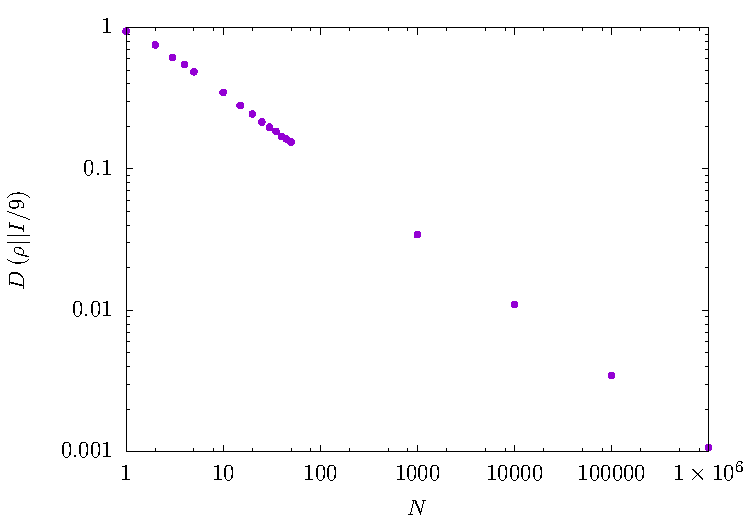
\includegraphics[width=0.45\linewidth]{avg_dist}}\hspace{1.5em} \subfloat[Average values of both quantifiers of magic - $\mathcal M$ and $\mathcal N$, and the average percentage of states which lie in the stabilizer hull]{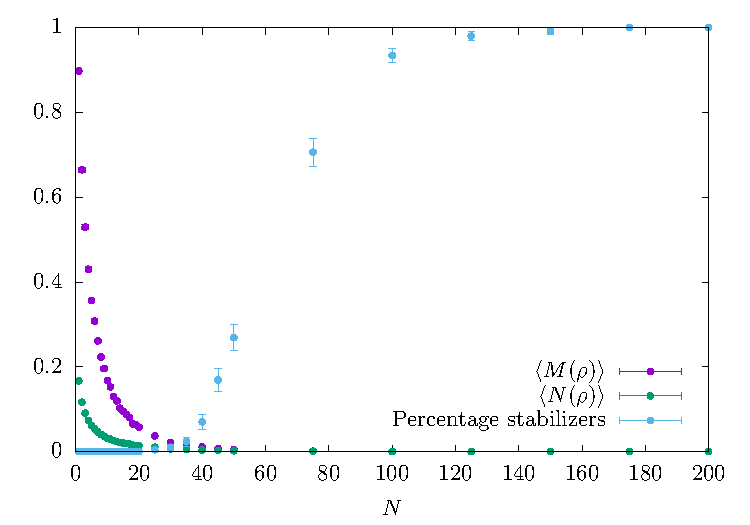
\includegraphics[width=0.45\linewidth]{avg_magic}}
\caption{Analysis of random state generation protocol as a function of the number $N$ of pure qudit states sampled in each mixed state. 100 mixed states were used to generate each point in the first plot, and 200 in the second. Error bars on both plots are generated using 100 bootstrap resamples - they are too small to see in the first plot.}
\end{figure}

\section{Efficient contraction scheme to compute $d(\rho,\sigma)$ and its derivatives}

\label{sec:contractions}

Let $\rho=\sum_{u,\alpha_i} \otimes_k\ \rho^{(k)u_k}_{\alpha_k\alpha_{k+1}} A_{u_k}$ and $\sigma=\sum_{u,\alpha_i} \otimes_k\ \sigma^{(k)u_k}_{\alpha_k\alpha_{k+1}} A_{u_k}$ be MPOs in the phase space basis $A_u$ \eqref{eq:phase_space_ops} with bond dimensions $D_\rho$ and $D_\sigma$, respectively. In this basis, the Wigner coefficients are simply given by the matrix products $W_u(\rho)=\prod_i \rho^{(i)u_i}$ and $W_u(\sigma)=\prod_i \sigma^{(i)u_i}$ due to \eqref{eq:wigner_repr}, and the distance between them when viewed as vectors in the Wigner function representation space is simply
\begin{equation}d(\rho,\sigma)=\left(\sum_u\left(\prod_i \rho^{(i)u_i}-\prod_j \rho^{(j)u_j}\right)^2\right)^{1/2}=d^{-n/2}\sqrt{\left<\rho|\rho\right>-2\left<\rho|\sigma\right>+\left<\sigma|\sigma\right>}\end{equation}
Where $\left<\rho|\sigma\right>$ denotes the Frobenius overlap between the states $\rho$ and $\sigma$\footnote{The factor of $d^{-n}$ comes from the normalization of the phase space operators \eqref{eq:phase_space_norm}}:
\begin{equation}\left<\rho|\sigma\right>=\Tr\left[\rho^\dagger\sigma\right]=d^{-n}\sum_u \left(\prod_i \rho^{(i)u_i}\right)\left(\prod_j \sigma^{(i)u_j}\right)\end{equation}
This overlap can be calculated using a contraction order which allows for only a linear number of computations in $d$ and $n$ and cubic in $D_\sigma$ and $D_\rho$:
\begin{figure}[H]
\centering
\includegraphics[width=0.7\linewidth]{{overlap_contraction}}
\end{figure}
In this diagram, vertical and horizontal lines indicate contraction over ``physical'' indices $u_i$ with dimension $d$ and ``bond'' indices with dimension $D_\rho$ (or $D_\sigma$), respectively. The tensor $M$ represents the tensor in memory during the contraction, which grows in size horizontally through the tensor network until all contractions are completed, at which point it contains no external legs and holds the value $\left<\rho|\sigma\right>$. The contractions in the diagram take $dD_\rho D_\sigma+dD_\rho^2 D_\sigma+dD_\rho D_\sigma^2+d D_\sigma D_\rho=\mathcal O(d D_\rho D_\sigma (D_\rho+D_\sigma))$ steps to compute. The entire calculation requires $n$ such contractions, and will take $O(n d D_\rho D_\sigma (D_\rho+D_\sigma))$ time.

The derivative of $d(\rho,\sigma)$ with respect to the matrix element $\sigma^{(i)a}_{\alpha\beta}$ requires the computation of the derivative of $\left<\rho|\sigma\right>$ with respect to $\sigma^{(i)a}_{\alpha\beta}$, which is given by the following tensor:
\begin{figure}[H]
\centering
\includegraphics[width=0.4\linewidth]{{derivative}}
\end{figure}
While this tensor as a function of $\alpha$, $a$, and $\beta$, can also be computed in linear time in $d$ using a similar contraction scheme, we can do even better by precomputing as much of it as we can before using it in the optimization procedure. This is done by contracting all of the tensors before and after $\rho^{(i)}$ into tensors $M_1$ and $M_2$ using the same procedure for calculating overlaps above, and then performing the final $\mathcal O(d D_\rho D_\sigma)$ contractions to group the three remaining tensors into one:
\begin{figure}[H]
\centering
\includegraphics[width=0.7\linewidth]{{derivative_contraction}}
\end{figure}
\bibliography{holography,ftqc_resource_theory,optimization}
\end{document}